\section{The derivative}
\subsection{Slope of a curve}
\[ \text{slope of the normal} = \frac{-1}{\text{slope of the tangent}} \]

\subsection{Properties of the derivative}
Here we give some properties of the derivative:
\begin{itemize}
\item The derivative is a linear operation:
\[ (f+g)'(x) = f'(x) + g'(x) \]
and
\[ (c\cdot f)'(x) = c\cdot f'(x) \qquad \forall c \in \R \]
\item \ueig{Product rule}
\[ (f\cdot g)'(x) = f(x)\cdot g'(x) + f'(x)g(x) \]
\item The derivative of $\frac{1}{f(x)}$, assuming $f(x) \neq 0$:
\[ \left(\frac{1}{f(x)}\right)' = \frac{f'(x)}{f(x)^2}. \]
\item Combining the previous two properties, we get the quotient rule (assuming $g(x)\neq 0$)
\[ \left(\frac{f(x)}{g(x)}\right)' = \frac{g(x)f'(x) - f(x)g'(x)}{g(x)^2}. \]
\item Finally we have the very important \ueig{chain rule}. This tells us how to take the derivative of composite functions:
\[ (f \circ g)'(x) = f'(g(x))g'(x). \]
We can also write this as
\[ \od{f(g(x))}{x} = \od{f}{g}\od{g}{x}. \]
TODO example
\item Derivative of an inverse
\[ \od{f^{-1}(x)}{x} = \frac{1}{f'(f^{-1}(x))} \]
\end{itemize}

TODO Faà di Bruno

\subsection{Derivatives of some common functions}
Using the results below together with the properties above we can calculate the derivative of a large number of functions.

\begin{itemize}
\item Let $n$ be an integer larger than or equal to $1$ and let $f(x) = x^n$. Then
\[ f'(x) = n x^{n-1}. \]
Using this result together with the property of linearity, we can easily calculate the derivative of any polynomial function. TODO: general exponent
\item The derivatives of the trigonometric functions can be derived from
\[ \sin'(x) = \cos \qquad \text{and} \qquad \cos'(x) = -\sin(x) \]
TODO: list
\item TODO cyclometric
\item TODO hyperbolic
\end{itemize}

\subsubsection{The exponential and logarithm}
Define natural logarithm $\ln$ and \textit{the} exponential function $\exp$.
\[ \od{\ln x}{x} = \frac{1}{x} \]
\[ a^x = e^{x\ln a} \qquad (a>0, x\in \R) \]

\[ e^x = \lim_{n\to \infty}\left(1+\frac{x}{n}\right)^n \]
and growth.

\subsection{L'Hôpital's rules}


\subsection{Higher order derivatives}
When we take the derivative of a function, we we get a new function. We can now take the derivative of this new function. This is called taking the second order derivative. This process can be repeated for as long as the derivatives exist. We write the $n$-th order derivative as
\[ f^{(n)}(x) = \od[n]{f}{n}. \]
So for example $f''(x) = f^{(2)}(x)$.

\subsection{Implicit differentiation}

\subsection{Partial derivatives}
\subsubsection{Definition}
\subsubsection{Geometric interpretation}

\subsection{Meaning of the differential $\diff{}$}
TODO conventional use + examples with nabla

TODO: put series here!

\subsection{Generalisations and types of derivatives}
TODO: Liebnitz rule!!! + linear.

\section{Integration}
TODO intuition, solving strategies, solving intelligently 
SEE: The electric field (first write all quantities, then )

TODO
Solving intelligently (later using physics): Green functions, method of mirrors (+ cfr. general section on equations)
charge distributions

separation of variables (Legendre polynomials)

going from discrete sum to integral (also opposite with dirac delta). volume int using $\mathcal{V}$ and surface $\mathcal{S}$

surface int goes to zero at infinity.


\subsection{Areas as limits of sums}
\subsubsection{Sums and sigma notation}
\subsubsection{Trapezoid rule}
\subsubsection{Midpoint rule}
\subsubsection{Simpson's rule}

\subsection{The definite integral}
\subsection{Computing different areas and volumes}
\subsubsection{Rotation bodies}
\subsubsection{Surface bounded by function of polar coordinate $\theta$}
\[ \frac{1}{2}\int_{\theta_1}^{\theta_2}[f(\theta)]^2\diff{\theta} \]

\subsection{The fundamental theorem of calculus}
\subsubsection{Indefinite integrals}
anti-derivative $+C$
\subsubsection{Some elementary integrals}

\subsection{Properties of integrals}
\subsubsection{Linearity}
\subsubsection{Mean-value theorem}
\subsubsection{Integrals of piece-wise continuous functions}

\subsection{Techniques of integration}
\subsubsection{Integrals of rational functions}
\subsubsection{Substitutions}
+ inverse substitutions
\subsubsection{Integration by parts}


\subsection{Improper integrals}


\subsection{Different types of integrals}
\subsubsection{Riemann}
\subsubsection{Lebesgue}
\subsubsection{Stieltjes}
\subsubsection{Cauchy}


\section{Graphs of functions}
\subsection{Scaling and translating}

\subsection{The parabola}
\begin{definition}
A \udef{parabola} is the graph of a second order real polynomial: $p:\R\to \R: x\mapsto ax^2 + bx +c$.
Here $a\in\R\setminus\{0\}$ and $b,c\in \R$.

We call $p$ the \udef{unit parabola} if $a = 1$ and $b= 0 =c$.
\end{definition}
TODO: definition by conic section or from point and line: the points on the parabola are equidistant to both the focus and the directrix.

\begin{figure}[h!]
\centering
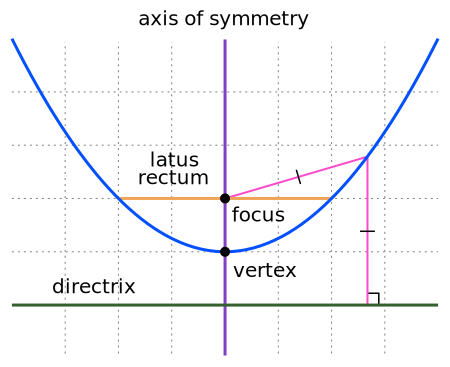
\includegraphics[width=.8\textwidth]{Parts_of_Parabola}
\caption{Parts of parabola. By Melikamp - Own work, CC BY-SA 3.0, \url{https://commons.wikimedia.org/w/index.php?curid=28181019}. TODO: add focal length as distance from vertex to focus.}
\end{figure}

\begin{lemma}
Let $p(x) = ax^2 + bx +c$ be a parabola. Then we have
\begin{itemize}
\item the vertex $V = \Big(-\frac{b}{2a}, \frac{4ac - b^2}{4a}\Big)$;
\item the focus $F = \Big(-\frac{b}{2a}, \frac{4ac - b^2+1}{4a}\Big)$;
\item the directrix $y = \frac{4ac - b^2 -1}{4a}$;
\item the semi-latus rectum is $\frac{1}{2a}$.
\end{itemize}
Note the focal length is $\frac{1}{4a}$.
\end{lemma}


\begin{lemma}
Every parabola can be transformed into the unit parabola by translation and uniform scaling.
\end{lemma}

\section{Silly integrals}
\[ \int x^{\diff x}-1 = x\ln(x) - x +c \]